\chapter{Perancangan}
\label{chap:perancangan}

Bab ini membahas tentang perancangan setiap fitur yang diimplementasi pada perangkat lunak \textit{Sharif Judge}. 

\section{Mengganti Method \textit{shell\_exec("rm ...")} Menjadi \textit{unlink()}}
\textit{Method} \textit{shell\_exec("rm ...")} yang memiliki fungsi untuk menghapus sebuah \textit{file} terdapat pada kelas \textit{controller Assignment.php} tepatnya di baris kode 425 dan 473

\textit{Assignments.php}
\begin{lstlisting}[basicstyle=\ttfamily, frame=single,
columns=fullflexible, keepspaces=true]
...
423	// Upload Tests (zip file)
424	
425	shell_exec('rm -f '.$assignments_root.'/*.zip');
426	$config = array(
...
472	foreach($old_pdf_files as $old_name)
473		shell_exec("rm -f $old_name");
474	$this->messages[] = array(
...
\end{lstlisting}

Fungsi \textit{shell\_exec("rm ...")} pada baris 425 dan 473 diubah menggunakan fungsi \textit{unlink()} menjadi seperti berikut

\textit{Assignments.php}
\begin{lstlisting}[basicstyle=\ttfamily, frame=single,
columns=fullflexible, keepspaces=true]
...
423	// Upload Tests (zip file)
424	
425	unlink($assignments_root.'/*.zip');
426	$config = array(
...
472	foreach($old_pdf_files as $old_name)
473		unlink($old_name);
474	$this->messages[] = array(
...
\end{lstlisting}

\section{Menambahkan Method Rekoneksi ke \textit{Database}}
\textit{Method} rekoneksi ke \textit{database} ditambahkan pada kelas \textit{controller Queueprocess.php}. 

\textit{Queueprocess.php}
\begin{lstlisting}[basicstyle=\ttfamily, frame=single,
columns=fullflexible, keepspaces=true]
...
133
134	// Save the result
135	$this->queue_model->save_judge_result_in_db($submission, $type);
...
\end{lstlisting}

\textit{Method} rekoneksi yang digunakan yaitu \textit{\$this->db->reconnect()}. \textit{Method} ini diletakan pada baris 134 tepat sebelum \textit{Sharif Judge} menyimpan hasil \textit{judge}. Hal tersebut dilakukan untuk menghindari \textit{connection times out} akibat pengujian yang memakan waktu lama.

\textit{Queueprocess.php}
\begin{lstlisting}[basicstyle=\ttfamily, frame=single,
columns=fullflexible, keepspaces=true]
...
133
134	//reconnect to database incase we have run test for a long time.
135	$this->db->reconnect();
136
137	// Save the result
138	$this->queue_model->save_judge_result_in_db($submission, $type);
...
\end{lstlisting}

\section{Membatasi Soal (deskripsi \& PDF) Hanya Dapat Diunduh dengan Syarat Tertentu}%}Saat \textit{Assignment "Open"} dan setelah waktu mulai}
Fungsi untuk mengunduh soal (deskripsi \& PDF) terdapat pada \textit{controller Assignment.php} tepatnya di baris kode 100.

\textit{Assignments.php}
\begin{lstlisting}[basicstyle=\ttfamily, frame=single,
columns=fullflexible, keepspaces=true, breaklines=true]
...
97	/**
98	* Download pdf file of an assignment (or problem) to browser
99	*/
100	public function pdf($assignment_id, $problem_id = NULL)
101	{
102		// Find pdf file
103		if ($problem_id === NULL)
104			$pattern = rtrim($this->settings_model->get_setting('assignments_root'),'/')."/assignment_{$assignment_id}/*.pdf";
105		else
106			$pattern = rtrim($this->settings_model->get_setting('assignments_root'),'/')."/assignment_{$assignment_id}/p{$problem_id}/*.pdf";
107		$pdf_files = glob($pattern);
108		if ( ! $pdf_files )
109			show_error("File not found");
110
111		// Download the file to browser
112		$this->load->helper('download')->helper('file');
113		$filename = shj_basename($pdf_files[0]);
114		force_download($filename, file_get_contents($pdf_files[0]), TRUE);
115	}
...
\end{lstlisting}

Selain membatasi soal (deskripsi \& PDF) hanya dapat diunduh saat \textit{assignment "open"} dan setelah waktu mulai, pada fungsi ini juga ditambahkan fitur lain. Fitur lain tersebut yaitu membatasi soal hanya dapat diunduh oleh peserta yang terdaftar sebagai "\textit{participant}" dan soal tidak dapat diunduh setelah melewati batas waktu pengumpulan. Rancangan algoritma kode yang digunakan yaitu
\begin{itemize}
	\item Membuat atribut tambahan untuk menyimpan informasi waktu selesai, waktu mulai dan waktu tambahan sebuah assignment.
	\item Jika atribut "\textit{open}" pada \textit{assignment} tidak memiliki nilai, maka munculkan pesan \textit{error} "\textit{Selected assignment has been closed}."
	\item Jika pengguna tidak terdaftar sebagai "\textit{participant}" dalam \textit{assignment} yang dipilih, maka munculkan pesan error "\textit{You are not registered for submitting}."
	\item Jika waktu sekarang telah melewati batas waktu selesai + waktu tambahan, maka munculkan pesan \textit{error} "\textit{Selected assignment has finished}."
	\item Jika waktu sekarang belum melewati waktu mulai, maka munculkan pesan \textit{error} "\textit{Selected assignment has not started}."	
\end{itemize}

Berikut hasil pengimplementasian rancangan algoritma di atas ke dalam kode program

\textit{Assignments.php}
\begin{lstlisting}[basicstyle=\ttfamily, frame=single,
columns=fullflexible, keepspaces=true, breaklines=true]
...
97	/**
98	* Download pdf file of an assignment (or problem) to browser
99	*/
100	public function pdf($assignment_id, $problem_id = NULL)
101	{
102		$finishtime = strtotime($this->assignment_model->assignment_info($assignment_id)['finish_time']);
103		$starttime = strtotime($this->assignment_model->assignment_info($assignment_id)['start_time']);
104		$extratime = $this->assignment_model->assignment_info($assignment_id)['extra_time'];
105
106		// Find pdf file
107		if ($problem_id === NULL)
108			$pattern = rtrim($this->settings_model->get_setting('assignments_root'),'/')."/assignment_{$assignment_id}/*.pdf";
109		else
110			$pattern = rtrim($this->settings_model->get_setting('assignments_root'),'/')."/assignment_{$assignment_id}/p{$problem_id}/*.pdf";
111		$pdf_files = glob($pattern);
112		if ( ! $pdf_files )
113			show_error("File not found");
114		elseif (!$this->assignment_model->assignment_info($assignment_id)['open'])
115			show_error('Selected assignment has been closed.');
116		elseif	( ! $this->assignment_model->is_participant($this->assignment_model->assignment_info($assignment_id)['participants'],$this->user->username) )
117			show_error('You are not registered for submitting.');
118		elseif ( shj_now() > $finishtime + $extratime)
119			show_error('Selected assignment has finished.');
120		elseif ( shj_now() < $starttime)
121			show_error('Selected assignment has not started.');
122			
123		// Download the file to browser
124		$this->load->helper('download')->helper('file');
125		$filename = shj_basename($pdf_files[0]);
126		force_download($filename, file_get_contents($pdf_files[0]), TRUE);
127	}
...
\end{lstlisting}

\section{Mensupport \textit{File} dengan Ekstensi TXT}
Untuk dapat mensupport \textit{file} dengan ekstensi TXT pada perangkat lunak \textit{Sharif Judge}, diperlukan penambahan dan perubahan kode pada beberapa kelas. Beberapa kelas tersebut antara lain \textit{controller Submit.php, model Assignment\_model.php, view submissions.twig} dan kelas bantuan \textit{shj\_helper.php} yang terdapat pada direktori \path{Sharif-Judge\application\helper}. Berikut beberapa baris potongan kode program

\textit{Submit.php}
\begin{lstlisting}[basicstyle=\ttfamily, frame=single,
columns=fullflexible, keepspaces=true, breaklines=true]
...
58		case 'java': return 'java';
59		case 'zip': return 'zip';
60		case 'pdf': return 'pdf';
61		default: return FALSE;
62	}
...
76		case 'java': return ($extension==='java'?TRUE:FALSE);
77		case 'zip': return ($extension==='zip'?TRUE:FALSE);
78		case 'pdf': return ($extension==='pdf'?TRUE:FALSE);
79	}
...
88	if ($str=='0')
89		return FALSE;
90	if (in_array( strtolower($str),array('c', 'c++', 'python 2', 'python 3', 'java', 'zip', 'pdf')))
91		return TRUE;
92	return FALSE;
...
\end{lstlisting}

\textit{Assignment\_model.php}
\begin{lstlisting}[basicstyle=\ttfamily, frame=single,
columns=fullflexible, keepspaces=true, breaklines=true]
...
100	$item2 = strtolower($item);
101	if ( ! in_array($item2, array('c','c++','python 2','python 3','java','zip','pdf')))
102		continue;
...
\end{lstlisting}

\textit{shj\_helper.php}
\begin{lstlisting}[basicstyle=\ttfamily, frame=single,
columns=fullflexible, keepspaces=true, breaklines=true]
...
81	case 'java': return 'java';
82	case 'zip': return 'zip';
83	case 'pdf': return 'pdf';
84	default: return FALSE;
...
104	case 'java': return 'Java';
105	case 'zip': return 'Zip';
106	case 'pdf': return 'PDF';
107	default: return FALSE;
...
\end{lstlisting}

\textit{submissions.twig}
\begin{lstlisting}[basicstyle=\ttfamily, frame=single,
columns=fullflexible, keepspaces=true, breaklines=true]
...
160	<td>
161		
162			<div class="btn shj-orange" data-type="download">Download</div>
163		
164			<div class="btn shj-orange" data-type="code" >Code</div>
165		
166	</td>
...
\end{lstlisting}

Penambahan dan perubahan kode dilakukan setelah baris 60, 78 dan 90 pada \textit{controller Submit.php}. Berikut hasil penambahan dan perubahan kode 

\textit{Submit.php}
\begin{lstlisting}[basicstyle=\ttfamily, frame=single,
columns=fullflexible, keepspaces=true, breaklines=true]
...
58		case 'java': return 'java';
59		case 'zip': return 'zip';
60		case 'pdf': return 'pdf';
61		case 'txt': return 'txt';
62		default: return FALSE;
63	}
...
77		case 'java': return ($extension==='java'?TRUE:FALSE);
78		case 'zip': return ($extension==='zip'?TRUE:FALSE);
79		case 'pdf': return ($extension==='pdf'?TRUE:FALSE);
80		case 'txt': return ($extension==='txt'?TRUE:FALSE);
81	}
...
90	if ($str=='0')
91		return FALSE;
92	if (in_array( strtolower($str),array('c', 'c++', 'python 2', 'python 3', 'java', 'zip', 'pdf', 'txt')))
93		return TRUE;
94	return FALSE;
...
\end{lstlisting}

Perubahan kode dilakukan di baris 101 pada model \textit{Assignment\_model.php}. Berikut hasil perubahan kode 

\textit{Assignment\_model.php}
\begin{lstlisting}[basicstyle=\ttfamily, frame=single,
columns=fullflexible, keepspaces=true, breaklines=true]
...
100	$item2 = strtolower($item);
101	if ( ! in_array($item2, array('c','c++','python 2','python 3','java','zip','pdf','txt')))
102		continue;
...
\end{lstlisting}

Penambahan kode dilakukan setelah baris 83 pada kelas bantuan \textit{shj\_helper.php}. Berikut hasil penambahan kode 

\textit{shj\_helper.php}
\begin{lstlisting}[basicstyle=\ttfamily, frame=single,
columns=fullflexible, keepspaces=true, breaklines=true]
...
81	case 'java': return 'java';
82	case 'zip': return 'zip';
83	case 'pdf': return 'pdf';
84	case 'txt': return 'txt';
85	default: return FALSE;
...
105	case 'java': return 'Java';
106	case 'zip': return 'Zip';
107	case 'pdf': return 'PDF';
108	case 'txt': return 'TXT';
109	default: return FALSE;
...
\end{lstlisting}

Perubahan kode dilakukan pada baris 161 pada \textit{view submissions.twig}. Berikut hasil perubahan kode

\textit{submissions.twig}
\begin{lstlisting}[basicstyle=\ttfamily, frame=single,
columns=fullflexible, keepspaces=true, breaklines=true]
...
160	<td>
161		
162			<div class="btn shj-orange" data-type="download">Download</div>
163		
164			<div class="btn shj-orange" data-type="code" >Code</div>
165		
166	</td>
...
\end{lstlisting}

\section{Menambahkan Halaman \textit{Logs}}% yang Mencatat Aktivitas \textit{Login} Pengguna}
Agar halaman \textit{Logs} dapat berjalan dengan baik, perlu ditambahkan tabel baru pada \textit{database} \textit{Sharif Judge}.  \textit{Tabel} baru tersebut bernama \textit{shj\_logins}. 
\begin{table}[H] %atau h saja untuk "kira kira di sini"
	\centering 
	\caption{Perancangan Tabel \textit{shj\_logins}}
	\label{tab:tabellogs}
		\begin{tabular}{|c|c|c|c|}
			\hline
			\textbf{Atribut} & \textbf{Tipe Data} & \textbf{Ukuran}  & \textbf{Default} \\
			\hline
			\textit{login\_id (primary key)} & int & 11  & None \\
			\hline
			\textit{username} & varchar & 20  & None \\
			\hline
			\textit{ip\_address} & varchar & 15  & None \\
			\hline
			\textit{timestamp} & timestamp & 11  & current\_timestamp \\
			\hline
			\textit{last\_24h\_login\_id}	 & int & 11  & null \\
			\hline
		\end{tabular}
\end{table}

Keterangan atribut:
\begin{enumerate}
	\item \textit{login\_id}: sebagai penanda yang membedakan setiap \textit{login} peserta satu dengan yang lain. Memiliki \textit{length default} int dari \textit{phpMyAdmin} yaitu 11. Atribut \textit{login\_id} merupakan \textit{primary key} karena id harus unik agar setiap \textit{login} peserta dapat dibedakan. Atribut ini juga bersifat \textit{auto increment}.
	\item \textit{username}: \textit{username} peserta yang berhasil \textit{login} pada \textit{Sharif Judge}. Memiliki \textit{length varchar} 20 karena \textit{length username} pada tabel \textit{shj\_users} adalah 20.
	\item \textit{ip\_address}: \textit{ip address} peserta yang berhasil \textit{login} pada \textit{Sharif Judge}. Memiliki \textit{length varchar} 15 karena \textit{length} maksimal dari \textit{ip address protocol version 4 (IPv4)} adalah 15. Contoh: 202.100.123.255
	\item \textit{timestamp}: waktu peserta saat berhasil \textit{login} pada \textit{Sharif Judge}. Menggunakan tipe data timestamp yang mencatat waktu \textit{login} dengan format YYYY-MM-DD HH:MM:SS. Contoh: 2018-04-06 18:15:43
	\item \textit{last\_24h\_login\_id}: id \textit{login} peserta yang berhasil \textit{login} pada \textit{Sharif Judge} namun menggunakan \textit{ip address} berbeda dalam waktu 24 jam terakhir.
\end{enumerate}

Selain tabel diatas, halaman logs juga ditambahkan kelas \textit{model, view} dan \textit{controller}.
\begin{enumerate}
	\item \textit{Model} \\
	\textit{Model} untuk halaman \textit{logs} bernama \textit{Logs\_model.php}. Berikut adalah perincian fungsi yang terdapat dalam rancangan \textit{model Logs\_model.php}.
	\begin{table}[H]
		\caption{Perincian fungsi \textit{insert\_to\_logs}}
		\begin{tabular}{|c|p{11cm}|}
			\hline
			Nama \textit{Method} 	& 	\textit{insert\_to\_logs} 	\\
			\hline
			Parameter \textit{Input} & \textit{\$username} dan \textit{\$ip\_address} \\
			\hline
			Parameter \textit{Output} & -\\
			\hline
			Tabel yang berhubungan & \textit{shj\_logins} \\
			\hline
			Deskripsi	& Proses untuk memasukan \textit{logs} pengguna \textit{Sharif Judge} \\
			\hline
			Algoritma	& \begin{itemize}
				\item Mengecek dan menghapus \textit{logs} pada tabel \textit{shj\_logins} yang \textit{timestampnya} lebih dari 24 jam.
				\item Mengecek entri \textit{login} terakhir untuk \textit{\$username} yang  menggunakan \textit{IP address} tidak sama dengan \textit{\$ip\_address}
				\item Jika tidak memiliki hasil, maka tambahkan entri baru menggunakan \textit{\$username} dan \textit{\$ip\_address} tersebut.
				\item Jika memiliki hasil,  maka tambahkan entri baru menggunakan \textit{\$username} dan \textit{\$ip\_address} serta. last\textit{\_24h\_login\_id} diisi dengan \textit{login\_id} sebelumnya
			\end{itemize} \\
			\hline
		\end{tabular}
	\end{table}

	\begin{table}[H]
		\caption{Perincian fungsi \textit{get\_all\_logs}}
		\begin{tabular}{|c|p{11cm}|}
			\hline
			Nama \textit{Method} 	& 	\textit{get\_all\_logs} 	\\
			\hline
			Parameter \textit{Input} & - \\
			\hline
			Parameter \textit{Output} &  semua entri logs dari tabel \textit{shj\_logins}\\
			\hline
			Tabel yang berhubungan & \textit{shj\_logins} \\
			\hline
			Deskripsi	& Proses untuk mengembalikan entri \textit{logs} yang terdapat pada tabel \textit{shj\_logins} \\
			\hline
			Algoritma	& \begin{itemize}
				\item Mengembalikan seluruh entri logs yang terdapat pada tabel \textit{shj\_logins} dalam bentuk \textit{array}.
			\end{itemize} \\
			\hline
		\end{tabular}
	\end{table}

	\item View \\
	\textit{View} untuk halaman \textit{logs} bernama \textit{logs.twig}. Menu halaman \textit{logs} terletak di paling bawah menu lainnya dan bernama '\textit{24-hour log}'. Berikut adalah rancangan tampilan halaman \textit{logs}.
	
	\begin{figure}[H]
		\centering  
		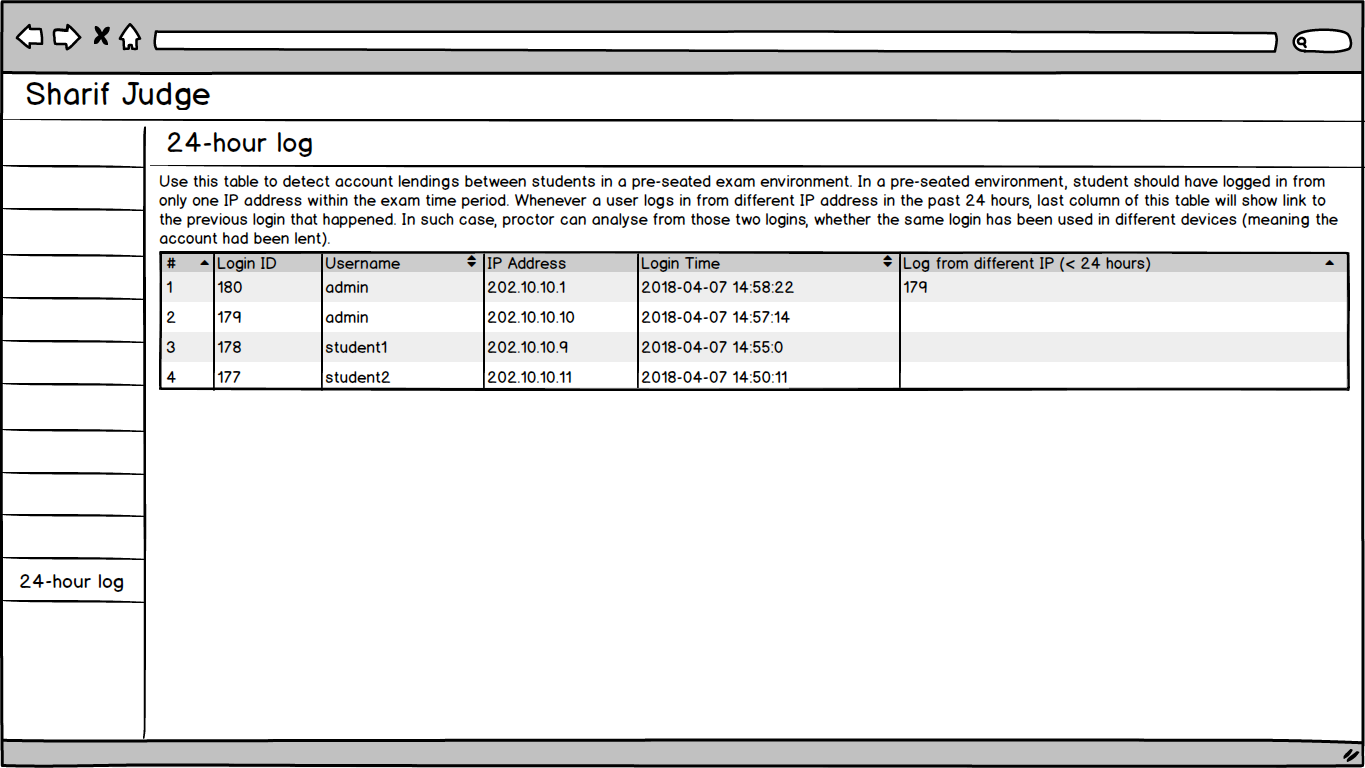
\includegraphics[width=1.0\textwidth]{mockuplogs}  
		\caption[Rancangan tampilan halaman \textit{logs}]{Rancangan tampilan halaman \textit{logs}} 
		\label{fig:mockuplogs} 
	\end{figure}

	\item \textit{Controller} \\
	\textit{Controller} untuk halaman \textit{logs} bernama \textit{Logs.php}. Berikut adalah perincian fungsi yang terdapat dalam rancangan \textit{controller Logs.php}.
	\begin{table}[H]
		\caption{Perincian fungsi \textit{consturct\_\_}}
		\begin{tabular}{|c|p{11cm}|}
			\hline
			Nama \textit{Method} 	& 	\textit{consturct\_\_} 	\\
			\hline
			Parameter \textit{Input} & - \\
			\hline
			Parameter \textit{Output} &  - \\
			\hline
			Tabel yang berhubungan & - \\
			\hline
			Deskripsi	& membatasi pengguna yang dapat mengakses halaman \textit{logs}	 \\
			\hline
			Algoritma	& \begin{itemize}
				\item Mengecek \textit{session} pengguna yang akan mengakses halaman \textit{logs}.
				\item Jika \textit{session} tidak berstatus '\textit{logged\_in}, maka pengguna akan dialihkan ke halaman \textit{login}.
				\item Mengecek \textit{role} pengguna yang akan mengakses halaman \textit{logs}.
				\item Jika role pengguna bukan \textit{admin}, maka pengguna akan dialihkan ke halaman \textit{'404 Not Found'}.
			\end{itemize} \\
			\hline
		\end{tabular}
	\end{table}
	
	\begin{table}[H]
		\caption{Perincian fungsi \textit{index}}
		\begin{tabular}{|c|p{11cm}|}
			\hline
			Nama \textit{Method} 	& 	\textit{index} 	\\
			\hline
			Parameter \textit{Input} & - \\
			\hline
			Parameter \textit{Output} &  - \\
			\hline
			Tabel yang berhubungan & \textit{shj\_logins} \\
			\hline
			Deskripsi	& Proses untuk memuat seluruh entri \textit{logs} pada halaman \textit{logs.twig}	 \\
			\hline
			Algoritma	& \begin{itemize}
				\item Memuat data \textit{logs} menggunakan fungsi \textit{get\_all\_logs} dari \textit{model Logs\_model.php}.
				\item Memproses data untuk tampilan \textit{logs.twig}.
			\end{itemize} \\
			\hline
		\end{tabular}
	\end{table}
\end{enumerate}

\section{Menambahkan Parameter "\textit{Display Name}" pada Pendaftaran Peserta \textit{Sharif Judge}}
Untuk dapat menambahkan parameter "\textit{Display Name}" pada pendaftaran peserta \textit{Sharif Judge}, diperlukan beberapa perubahan dan penambahan kode. Berikut rancangan algoritma yang dilakukan
\begin{enumerate}
	\item Menambahkan parameter "\textit{Display Name}" pada fungsi \textit{add\_user} yang terdapat di \textit{model User\_model.php}.
	\item Mengubah pemisah (\textit{separator}) antar parameter pada fungsi \textit{add\_user}. Pemisah antar parameter yang awalnya menggunakan spasi diubah menggunakan tanda koma.
	\item Menambahkan keterangan parameter "\textit{Display Name}" pada halaman \textit{add\_user.twig} dan  \textit{add\_user\_result.twig}.
	\item Menambahkan \textit{Display Name} untuk \textit{admin} pada proses \textit{install Sharif Judge}.
	\item Mengubah urutan data yang digunakan pada fungsi pendaftaran peserta melalui \textit{email}.
	\item Menambahkan \textit{text field Display Name} pada halaman \textit{Register} \textit{(Open Public Registration}).
\end{enumerate}
Dari rancangan algoritma yang diterapkan, terdapat perubahan dan penambahan kode pada beberapa kelas. Beberapa kelas tersebut antara lain \textit{controller Install.php, controller Login.php, model User\_model.php, view add\_user.twig, view add\_user\_result.twig} dan \textit{view register.twig}.
Berikut beberapa baris potongan kode program

\textit{Install.php}
\begin{lstlisting}[basicstyle=\ttfamily, frame=single,
columns=fullflexible, keepspaces=true, breaklines=true]
...
252	// add admin user
253	$this->user_model->add_user(
254		$this->input->post('username'),
255		$this->input->post('email'),
256		$this->input->post('password'),
257		'admin'
	);
...
\end{lstlisting}
~\\
\textit{Login.php}
\begin{lstlisting}[basicstyle=\ttfamily, frame=single,
columns=fullflexible, keepspaces=true, breaklines=true]
...
92	$this->user_model->add_user(
93		$this->input->post('username'),
94		$this->input->post('email'),
95		$this->input->post('password'),
...
\end{lstlisting}
~\\
\textit{User\_model.php}
\begin{lstlisting}[basicstyle=\ttfamily, frame=single,
columns=fullflexible, keepspaces=true, breaklines=true]
...
120	*/
121	public function add_user($username, $email, $password, $role)
122	{
...
138	'username' => $username,
139	'email' => $email,
140	'password' => $this->password_hash->HashPassword($password),
...
176	$parts = preg_split('/\s+/', $line);
177	if (count($parts) != 4)
178		continue; //ignore lines that not contain 4 parts
...
180	if (strtolower(substr($parts[2], 0, 6)) == 'random')
181	{
182		// generate random password
183		$len = trim(substr($parts[2], 6), '[]');
184		if (is_numeric($len)){
185			$this->load->helper('string');
186			$parts[2] = shj_random_password($len);
187		}
188	}
189	
190	$result = $this->add_user($parts[0], $parts[1], $parts[2], $parts[3]);
191	
192	if ($result === TRUE)
193		array_push($users_ok, array($parts[0], $parts[1], $parts[2], $parts[3]));
194	else
195		array_push($users_error, array($parts[0], $parts[1], $parts[2], $parts[3], $result));
...
230	$text = str_replace('{SITE_URL}', base_url(), $text);
231	$text = str_replace('{ROLE}', $user[3], $text);
232	$text = str_replace('{USERNAME}', $user[0], $text);
233	$text = str_replace('{PASSWORD}', htmlspecialchars($user[2]), $text);
234	$text = str_replace('{LOGIN_URL}', base_url(), $text);
...
\end{lstlisting}
~\\
\textit{add\_user.twig}
\begin{lstlisting}[basicstyle=\ttfamily, frame=single,
columns=fullflexible, keepspaces=true, breaklines=true]
...
66	#
67	# USERNAME EMAIL PASSWORD ROLE
68	#
...
\end{lstlisting}
~\\
\textit{add\_user\_result.twig}
\begin{lstlisting}[basicstyle=\ttfamily, frame=single,
columns=fullflexible, keepspaces=true, breaklines=true]
...
9	
10	<li>Usename: {{ item[0] }} Email: {{ item[1] }} Password: <code>{{ item[2] }}</code> Role: {{ item[3] }}</li>
11	
...
17	
18	<li>Usename: {{ item[0] }} Email: {{ item[1] }} Password: <code>{{ item[2] }}</code> Role: {{ item[3] }} ({{ item[4] }})</li>
19	
...
\end{lstlisting}
~\\
\textit{register.twig}
\begin{lstlisting}[basicstyle=\ttfamily, frame=single,
columns=fullflexible, keepspaces=true, breaklines=true]
...
33	{{ form_error('email','<div class="shj_error">','</div>') }}
34	</p>
35	<p>
36	<label for="form_password">Password</label><br/>
...
\end{lstlisting}
~\\
Perubahan dan penambahan kode di \textit{User\_model.php} untuk menambahkan parameter "\textit{Display Name}". Penambahan kode tersebut terjadi pada baris 121, 139, 180, 183, 190, 193 dan 195. Mengubah pemisah antar parameter menggunakan tanda koma terjadi pada baris 176. Mengubah urutan data pada pada pendaftaran peserta melalui \textit{email} terjadi pada baris 231 dan 233. Berikut hasil penambahan dan perubahan kode program yang terjadi di \textit{User\_model.php}

\textit{User\_model.php}
\begin{lstlisting}[basicstyle=\ttfamily, frame=single,
columns=fullflexible, keepspaces=true, breaklines=true]
...
120	*/
121	public function add_user($username, $email, $display_name, $password, $role)
122	{
...
138	'username' => $username,
139	'email' => $email,
140	'display_name' => $display_name,
141	'password' => $this->password_hash->HashPassword($password),
...
177	$parts = preg_split('/,+/', $line);
178	if (count($parts) != 5)
179		continue; //ignore lines that not contain 5 parts
...
181	if (strtolower(substr($parts[3], 0, 6)) == 'random')
182	{
183		// generate random password
184		$len = trim(substr($parts[3], 6), '[]');
185		if (is_numeric($len)){
186			$this->load->helper('string');
187			$parts[3] = shj_random_password($len);
188		}
189	}
190	
191	$result = $this->add_user($parts[0], $parts[1], $parts[2], $parts[3]);
192	
193	if ($result === TRUE)
194		array_push($users_ok, array($parts[0], $parts[1], $parts[2], $parts[3], $parts[4]));
195	else
196		array_push($users_error, array($parts[0], $parts[1], $parts[2], $parts[3], $parts[4], $result));
...
231	$text = str_replace('{SITE_URL}', base_url(), $text);
232	$text = str_replace('{ROLE}', $user[4], $text);
233	$text = str_replace('{USERNAME}', $user[0], $text);
234	$text = str_replace('{PASSWORD}', htmlspecialchars($user[3]), $text);
235	$text = str_replace('{LOGIN_URL}', base_url(), $text);
...
\end{lstlisting}
~\\
Penambahan kode di \textit{Install.php} untuk menambahkan \textit{Display Name admin} terjadi setelah baris 255. Berikut hasil penambahan kode program yang terjadi di \textit{Install.php}
 
\textit{Install.php}
\begin{lstlisting}[basicstyle=\ttfamily, frame=single,
columns=fullflexible, keepspaces=true, breaklines=true]
...
252	// add admin user
253	$this->user_model->add_user(
254		$this->input->post('username'),
255		$this->input->post('email'),
256		'Admin',
257		$this->input->post('password'),
258		'admin'
);
...
\end{lstlisting}
~\\ 
Perubahan dan penambahan kode di halaman \textit{add\_user.twig} untuk menambahkan keterangan parameter "\textit{Display Name}". Penambahan kode tersebut terjadi pada baris 67, sedangkan halaman \textit{add\_user\_result.twig} terjadi pada baris 10 dan 18. Berikut hasil penambahan kode program yang terjadi di halaman \textit{add\_user.twig} dan halaman \textit{add\_user\_result.twig}

\textit{add\_user.twig}
\begin{lstlisting}[basicstyle=\ttfamily, frame=single,
columns=fullflexible, keepspaces=true, breaklines=true]
...
66	#
67	# USERNAME,EMAIL,DISPLAY-NAME,PASSWORD,ROLE
68	#
...
\end{lstlisting}

\textit{add\_user\_result.twig}
\begin{lstlisting}[basicstyle=\ttfamily, frame=single,
columns=fullflexible, keepspaces=true, breaklines=true]
...
9	
10	<li>Usename: {{ item[0] }} Email: {{ item[1] }} Diplay Name: {{ item[2] }} Password: <code>{{ item[3] }}</code> Role: {{ item[4] }} </li>
11	
...
17	
18	<li>Usename: {{ item[0] }} Email: {{ item[1] }} Diplay Name: {{ item[2] }} Password: <code>{{ item[3] }}</code> Role: {{ item[4] }} ({{ item[5] }})</li>
19	
...
\end{lstlisting}
~\\
Penambahan kode di halaman \textit{register.twig} untuk menambahkan \textit{text field Display Name} terjadi setelah baris 34 dan pada \textit{controller Login.php} setelah baris 94. Berikut hasil penambahan kode program yang terjadi di halaman \textit{register.twig} dan \textit{controller Login.php}.

\textit{register.twig}
\begin{lstlisting}[basicstyle=\ttfamily, frame=single,
columns=fullflexible, keepspaces=true, breaklines=true]
...
33	{{ form_error('email','<div class="shj_error">','</div>') }}
34	</p>
35	<p>
36		<label for="form_displayname">Display Name</label><br/>
37		<input id="form_displayname" type="text" name="displayname" required="required" pattern="[A-Za-z\s]+" title="The Display Name field must be contain only alphabetical letters" class="sharif_input" value="{{ set_value('displayname') }}"/>
38		{{ form_error('form_displayname', '<div class="shj_error">', '</div>') }}
39	</p>
40	<p>
41	<label for="form_password">Password</label><br/>
...
\end{lstlisting}

\textit{Login.php}
\begin{lstlisting}[basicstyle=\ttfamily, frame=single,
columns=fullflexible, keepspaces=true, breaklines=true]
...
92	$this->user_model->add_user(
93		$this->input->post('username'),
94		$this->input->post('email'),
95		$this->input->post('displayname'),
96		$this->input->post('password'),
...
\end{lstlisting}

\section{Menambahkan Fitur "\textit{Lock Student's Display Name}"}
Fitur "\textit{Lock Student's Display Name}" membutuhkan sebuah "\textit{key}" pada \textit{database}, dimana "\textit{key}" tersebut berfungsi untuk menyimpan sebuah nilai. Nilai yang disimpan akan menentukan apakah para peserta dapat mengubah \textit{Display Name} atau tidak. "\textit{Key}" disimpan pada tabel \textit{shj\_settings} pada kolom \textit{shj\_key} dengan nama \textit{lock\_student\_display\_name}. \textit{lock\_student\_display\_name} memiliki nilai \textit{default shj\_value} = 0. Jika nilai dari \textit{lock\_student\_display\_name} = 1, maka para peserta tidak dapat mengubah \textit{Display Name}, sebaliknya jika bernilai 0, maka para peserta dapat mengubah \textit{Display Name}.

Rancangan algoritma yang digunakan untuk menambahkan fitur "\textit{Lock Student's Display Name}" yaitu
\begin{enumerate}
	\item Menambahkan \textit{shj\_key} dengan nama \textit{lock\_student\_display\_name} yang memiliki nilai \textit{shj\_value} = 0 pada tabel \textit{shj\_settings}.
	\item Menambahkan \textit{check box} pada halaman \textit{settings.twig} untuk mengaktifkan atau menonaktifkan fitur "\textit{Lock Student's Display Name}".
	\item Jika fitur "\textit{Lock Student's Display Name}" diaktifkan, maka \textit{text field Display Name} pada halaman \textit{profile.twig} akan dinonaktifkan (\textit{disabled}).
	\item Jika fitur "\textit{Lock Student's Display Name}" dinonaktifkan, maka \textit{text field Display Name} pada halaman \textit{profile.twig} akan kembali aktif.
	\item Menambahkan fungsi untuk mengecek kembali nilai dari \textit{lock\_student\_display\_name} pada saat peserta menyimpan perubahan yang terjadi di halaman \textit{profile.twig}. Hal tersebut dilakukan untuk menangani para peserta yang "memaksa" agar dapat mengubah \textit{Display Name} dengan cara \textit{inspect element} lalu menghapus kode "\textit{disabled}" pada \textit{text field Display Name}.
\end{enumerate}

Dari rancangan algoritma yang diterapkan, terdapat penambahan kode pada beberapa kelas. Beberapa kelas tersebut antara lain \textit{controller Profile.php, controller Settings.php, model User\_model.php, view settings.twig} dan \textit{view profile.twig}.
Berikut beberapa baris potongan kode program

\textit{Profile.php}
\begin{lstlisting}[basicstyle=\ttfamily, frame=single,
columns=fullflexible, keepspaces=true, breaklines=true]
...
65		'role' => $user->role,
66		'form_status' => $this->form_status,
67	);
...
\end{lstlisting}
~\\
\textit{Settings.php}
\begin{lstlisting}[basicstyle=\ttfamily, frame=single,
columns=fullflexible, keepspaces=true, breaklines=true]
...
113	'results_per_page_all' => $this->input->post('rpp_all'),
114	'results_per_page_final' => $this->input->post('rpp_final'),
115	'week_start' => $this->input->post('week_start'),
...
\end{lstlisting}
~\\
\textit{User\_model.php}
\begin{lstlisting}[basicstyle=\ttfamily, frame=single,
columns=fullflexible, keepspaces=true, breaklines=true]
...
405	$username = $the_user->username;
406
407	$user=array(
408		'display_name' => $this->input->post('display_name'),
409		'email' => $this->input->post('email')
410	);
...
\end{lstlisting}
~\\
\textit{settings.twig}
\begin{lstlisting}[basicstyle=\ttfamily, frame=single,
columns=fullflexible, keepspaces=true, breaklines=true]
...
115		<span class="form_comment">Enable Log</span>
116	</p>
117	<p class="input_p">
...
\end{lstlisting}
~\\
\textit{profile.twig}
\begin{lstlisting}[basicstyle=\ttfamily, frame=single,
columns=fullflexible, keepspaces=true, breaklines=true]
...
31		<input id="form_name" type="text" name="display_name" class="sharif_input medium" value="{{ display_name }}"/>
32		{{ form_error('display_name', '<div class="shj_error">', '</div>') }}
33	</p>
...
\end{lstlisting}
~\\
Penambahan kode di halaman \textit{settings.twig} untuk menambahkan check box fitur "\textit{Lock Student's Display Name}". Penambahan kode tersebut terjadi setelah baris 116. Berikut hasil penambahan kode program yang terjadi di halaman \textit{settings.twig}

\textit{settings.twig}
\begin{lstlisting}[basicstyle=\ttfamily, frame=single,
columns=fullflexible, keepspaces=true, breaklines=true]
...
115		<span class="form_comment">Enable Log</span>
116	</p>
117	<p class="input_p">
118		<input id="form_lock_student_display_name" type="checkbox" name="lock_student_display_name" value="1" {{ lock_student_display_name ? 'checked' }}/>
119		<label for="form_lock_student_display_name">Lock Student's Display Name</label><br>
120		<span class="form_comment">Student's can't change their display name</span>
121	</p>
122	<p class="input_p">
...
\end{lstlisting}
~\\
Penambahan kode di \textit{controller Settings.php} untuk menyimpan nilai dari \textit{check box} fitur "\textit{Lock Student's Display Name}" ke \textit{database}. Penambahan kode tersebut terjadi setelah baris 115. Berikut hasil penambahan kode program yang terjadi di \textit{controller Settings.php}

\textit{Settings.php}
\begin{lstlisting}[basicstyle=\ttfamily, frame=single,
columns=fullflexible, keepspaces=true, breaklines=true]
...
113	'results_per_page_all' => $this->input->post('rpp_all'),
114	'results_per_page_final' => $this->input->post('rpp_final'),
115	'week_start' => $this->input->post('week_start'),
116	'lock_student_display_name' => $this->input->post('lock_student_display_name')===NULL?0:1,
...
\end{lstlisting}
~\\
Penambahan kode di \textit{controller Profile.php} untuk mengecek apakah fitur "\textit{Lock Student's Display Name}" aktif atau tidak aktif. Penambahan kode tersebut terjadi setelah baris 66. Hasil pengecekan tersebut akan dikirimkan untuk halaman \textit{profile.twig}. Berikut hasil penambahan kode program yang terjadi di \textit{controller} \textit{Profile.php}

\textit{Profile.php}
\begin{lstlisting}[basicstyle=\ttfamily, frame=single,
columns=fullflexible, keepspaces=true, breaklines=true]
...
65		'role' => $user->role,
66		'form_status' => $this->form_status,
67		'lock_student_display_name' => $this->settings_model->get_setting(lock_student_display_name),
68	);
...
\end{lstlisting}
~\\
Penambahan kode di halaman \textit{profile.twig} untuk menentukan apakah \textit{text field Display Name} akan diaktifkan atau tidak. Penambahan kode tersebut terjadi setelah baris 31. Berikut hasil penambahan kode program yang terjadi di tampilan \textit{profile.twig}

\textit{profile.twig}
\begin{lstlisting}[basicstyle=\ttfamily, frame=single,
columns=fullflexible, keepspaces=true, breaklines=true]
...
31
32	
33	<input id="form_name" type="text" name="display_name" class="sharif_input medium" value="{{ display_name }}" disabled/>
34	
35	<input id="form_name" type="text" name="display_name" class="sharif_input medium" value="{{ display_name }}"/>
36	
37
...
\end{lstlisting}
~\\
Penambahan kode di \textit{model User\_model.php} untuk mengecek apakah fitur "\textit{Lock Student's Display Name}" aktif atau tidak aktif. Penambahan kode tersebut terjadi setelah baris 405. Berikut hasil penambahan kode program yang terjadi di \textit{model User\_model.php}

\textit{User\_model.php}
\begin{lstlisting}[basicstyle=\ttfamily, frame=single,
columns=fullflexible, keepspaces=true, breaklines=true]

...
405	$username = $the_user->username;
406
407	$display_name = $this->input->post('display_name');
408	$locked = $this->settings_model->get_setting(lock_student_display_name);
409	if ($locked == 1) {
410		$display_name = $the_user->display_name;
411	}
412	
413	$user=array(
414		'display_name' => $display_name,
415		'email' => $this->input->post('email')
416	);
...
\end{lstlisting}

\section{Menambahakan Fitur "\textit{Archived Assignment}"}
Fitur "\textit{Archived Assignment}" membutuhkan sebuah atribut baru pada \textit{database}, dimana atribut tersebut berfungsi untuk menyimpan sebuah nilai. Nilai yang disimpan akan menentukan apakah \textit{assignment} tersebut bersifat \textit{Archived Assignment} atau tidak. Atribut baru tersebut  ditambahkan pada tabel \textit{shj\_assignments} dengan nama \textit{archived\_assignment} yang menggunakan tipe data \textit{tinyint}. \textit{archived\_assignment} memiliki nilai \textit{default} = 0. Jika nilai dari \textit{archived\_assignment} = 1, maka \textit{assignment} tersebut merupakan sebuah \textit{archived\_assignment}, sebaliknya jika bernilai 0, maka \textit{assignment} tersebut merupakan \textit{assignment} biasa.

Rancangan algoritma yang digunakan untuk menambahkan fitur "\textit{Archived Assignment}" yaitu
\begin{enumerate}
	\item Menambahkan atribut baru dengan nama \textit{archived\_assignment} yang menggunakan tipe data \textit{tinyint}. Atribut baru tersebut ditambahkan pada tabel \textit{shj\_assignments}
	\item Menambahkan \textit{check box} pada halaman \textit{assignments.twig} untuk mengaktifkan atau menonaktifkan fitur "\textit{Archived Assignment}".
	\item Jika fitur "\textit{Archived Assignment}" diaktifkan, maka secara otomatis \textit{text field Start time} bernilai 1970-01-02 00:00:00, \textit{text field Finish Time} bernilai 2038-01-18 00:00:00 dan \textit{text field Extra Time} bernilai 0.
	\item \textit{Assignment} yang bersifat \textit{Archived Assignment} tidak muncul pada kalendar halaman \textit{dashboard}.
\end{enumerate}

Dari rancangan algoritma yang diterapkan, terdapat penambahan kode pada beberapa kelas. Beberapa kelas tersebut antara lain \textit{model Assignment\_model.php, view add\_assignment.twig} dan \textit{view dashboard.twig}.
Berikut beberapa baris potongan kode program
~\\
\textit{Assignment\_model.php}
\begin{lstlisting}[basicstyle=\ttfamily, frame=single,
columns=fullflexible, keepspaces=true, breaklines=true]
...
37	foreach($extra_items as $extra_item)
38	{
39		$extra_time *= $extra_item;
40	}
41	$assignment = array(
42		'id' => $id,
43		'name' => $this->input->post('assignment_name'),
44		'problems' => $this->input->post('number_of_problems'),
45		'total_submits' => 0,
46		'open' => ($this->input->post('open')===NULL?0:1),
47		'scoreboard' => ($this->input->post('scoreboard')===NULL?0:1),
48		'javaexceptions' => ($this->input->post('javaexceptions')===NULL?0:1),
49		'description' => '', /* todo */
50		'start_time' => date('Y-m-d H:i:s', strtotime($this->input->post('start_time'))),
51		'finish_time' => date('Y-m-d H:i:s', strtotime($this->input->post('finish_time'))),
52		'extra_time' => $extra_time*60,
53		'late_rule' => $this->input->post('late_rule'),
54		'participants' => $this->input->post('participants')
55	);
...
\end{lstlisting}
~\\
\textit{add\_assignment.twig}
\begin{lstlisting}[basicstyle=\ttfamily, frame=single,
columns=fullflexible, keepspaces=true, breaklines=true]
...
37	$("#add").click(function(){
38			$('#problems_table>tbody').append(shj.row.replace(/PID/g, (shj.num_of_problems+1)));
39			shj.num_of_problems++;
40			$('#nop').attr('value', shj.num_of_problems);
41		});
42	$(document).on('click', '.delete_problem', function(){
43		if (shj.num_of_problems==1) return;
44		var row = $(this).parents('tr');
...
154		{{ form_error('javaexceptions', '<div class="shj_error">', '</div>') }}
155	</p>
156	<p class="input_p">
...
\end{lstlisting}
~\\
\textit{dashboard.twig}
\begin{lstlisting}[basicstyle=\ttfamily, frame=single,
columns=fullflexible, keepspaces=true, breaklines=true]
...
28	
29	
30		{id:{{ assignment.id }},title:'{{ assignment.name|e('js') }}', start:'{{ assignment.start_time }}', end:' {{ assignment.finish_time }}',
31		allDay:false,color:'{{ colors[(loop.index0)%colors|length] }}'}
32	,
33	
...
\end{lstlisting}
~\\
Penambahan kode di \textit{model Assignment\_model.php} untuk menyimpan nilai dari \textit{check box} fitur "\textit{Archived Assignment}" ke \textit{database}. Penambahan kode tersebut terjadi setelah baris 54. Penambahan kode setelah baris 40 berfungsi untuk mengambil nilai dari \textit{archived\_assignment} dari sebuah \textit{assignment}. Berikut hasil penambahan kode program yang terjadi di textit{model Assignment\_model.php} 

\textit{Assignment\_model.php}
\begin{lstlisting}[basicstyle=\ttfamily, frame=single,
columns=fullflexible, keepspaces=true, breaklines=true]
...
37	foreach($extra_items as $extra_item)
38	{
39		$extra_time *= $extra_item;
40	}
41
42	$archived_assignment = $archived_assignment = $this->input->post('archived_assignment')!==NULL ? 1 : 0;
43
44	$assignment = array(
45		'id' => $id,
46		'name' => $this->input->post('assignment_name'),
47		'problems' => $this->input->post('number_of_problems'),
48		'total_submits' => 0,
49		'open' => ($this->input->post('open')===NULL?0:1),
50		'scoreboard' => ($this->input->post('scoreboard')===NULL?0:1),
51		'javaexceptions' => ($this->input->post('javaexceptions')===NULL?0:1),
52		'description' => '', /* todo */
53		'start_time' => date('Y-m-d H:i:s', strtotime($this->input->post('start_time'))),
54		'finish_time' => date('Y-m-d H:i:s', strtotime($this->input->post('finish_time'))),
55		'extra_time' => $extra_time*60,
56		'late_rule' => $this->input->post('late_rule'),
57		'participants' => $this->input->post('participants')
58		'archived_assignment' => $archived_assignment
59	);
...
\end{lstlisting}
~\\
Penambahan kode di halaman \textit{add\_assignment.twig} untuk menambahkan \textit{check box} fitur "\textit{Archived Assignment}". Penambahan kode tersebut  terjadi setelah baris 155. Penambahan kode setelah baris 41 untuk mengisi nilai \textit{text field Start time} menjadi 1970-01-02 00:00:00, \textit{text field Finish Time} menjadi 2038-01-18 00:00:00 dan \textit{text field Extra Time} menjadi 0. Berikut hasil penambahan kode program yang terjadi di halaman \textit{add\_assignment.twig}

\textit{add\_assignment.twig}
\begin{lstlisting}[basicstyle=\ttfamily, frame=single,
columns=fullflexible, keepspaces=true, breaklines=true]
...
37	$("#add").click(function(){
38			$('#problems_table>tbody').append(shj.row.replace(/PID/g, (shj.num_of_problems+1)));
39			shj.num_of_problems++;
40			$('#nop').attr('value', shj.num_of_problems);
41		});
42	$("#form_a_archived_assignment").click(function(){
43		if ($("#form_a_archived_assignment").is(':checked')) {
44			$("#start_time").val('1970-01-02 00:00:00');
45			$("#finish_time").val('2038-01-18 00:00:00');
46			$("#form_extra_time").val('0');
47		}
48		else{
49			$("#start_time").val('');
50			$("#finish_time").val('');
51			$("#form_extra_time").val('');
52		}
53	});
54	$(document).on('click', '.delete_problem', function(){
55		if (shj.num_of_problems==1) return;
56		var row = $(this).parents('tr');
...
166		{{ form_error('javaexceptions', '<div class="shj_error">', '</div>') }}
167	</p>
168	<p class="input_p">
169		<input id="form_a_archived_assignment" type="checkbox" name="archived_assignment" value="1" {{ edit ? (edit_assignment.archived_assignment ? 'checked') : set_checkbox('archived_assignment', '1')|raw }} />
170		<label for="form_a_archived_assignment" class="default">Archived Assignment</label>
171		<span class="form_comment space-left">Check this to make an archived assignment</span>
172		{{ form_error('archived_assignment', '<div class="shj_error">', '</div>') }}
173	</p>
174	<p class="input_p">
...
\end{lstlisting}
~\\
Penambahan kode di halaman \textit{dashboard.twig} untuk mengatur \textit{assignment} yang bersifat \textit{Archived Assignment} agar tidak muncul pada kalendar. Penambahan kode tersebut terjadi setelah baris 29. Berikut hasil penambahan kode program yang terjadi di halaman \textit{dashboard.twig}

\textit{dashboard.twig}
\begin{lstlisting}[basicstyle=\ttfamily, frame=single,
columns=fullflexible, keepspaces=true, breaklines=true]
...
28	
29	
30		
31			{id:{{ assignment.id }},title:'{{ assignment.name|e('js') }}', start:'{{ assignment.start_time }}', end:' {{ assignment.finish_time }}', allDay:false,color:'{{ colors[(loop.index0)%colors|length] }}'}
32	
33		
34	{}
35	
36	,
37	
...
\end{lstlisting}

\section{Menambahkan Halaman \textit{Hall of Fame}}
Halaman \textit{Hall of Fame} tidak membutuhkan atribut atau tabel baru pada \textit{database} namun perlu ditambahkan \textit{model, view} dan \textit{controller}.

\begin{enumerate}
	\item \textit{Model} \\
	\textit{Model} untuk halaman \textit{Hall of Fame} bernama \textit{Hof\_model.php}. Berikut adalah perincian fungsi yang terdapat dalam rancangan \textit{model Hof\_model.php}.
	\begin{table}[H]
		\caption{Perincian fungsi \textit{get\_all\_final\_submission}}
		\begin{tabular}{|c|p{11cm}|}
			\hline
			Nama \textit{Method} 	& 	\textit{get\_all\_final\_submission} 	\\
			\hline
			Parameter \textit{Input} & - \\
			\hline
			Parameter \textit{Output} & semua entri nilai submissions yang telah dijumlahkan \\
			\hline
			Tabel yang berhubungan & \textit{shj\_submissions} \\
			\hline
			Deskripsi	& Proses untuk mengembalikan semua entri nilai submission yang telah djumlahkan pada tabel \textit{shj\_submissions} \\
			\hline
			Algoritma	& \begin{itemize}
				\item Menjumlahkan seluruh nilai submission setiap peserta yang tidak bersifat "\textit{Upload Only}". Nilai yang telah dijumlahkan akan disimpan sebagai total skor.
				\item Mengurutkan total skor dari yang paling besar.
				\item Mengembalikan seluruh entri yang telah dijumlahkan dalam bentuk \textit{array}.
			\end{itemize} \\
			\hline
		\end{tabular}
	\end{table}
	
	\begin{table}[H]
		\caption{Perincian fungsi \textit{get\_all\_user\_assignments}}
		\begin{tabular}{|c|p{11cm}|}
			\hline
			Nama \textit{Method} 	& 	\textit{get\_all\_user\_assignments} 	\\
			\hline
			Parameter \textit{Input} & \textit{\$username} \\
			\hline
			Parameter \textit{Output} &  mengembalikan seluruh \textit{details} dari \textit{assignment} pengguna tertentu\\
			\hline
			Tabel yang berhubungan & \textit{shj\_submissions} \\
			\hline
			Deskripsi	& Proses untuk mengembalikan \textit{details assignment} pengguna tertentu. \textit{Details} berisikan nama \textit{assignment}, nama \textit{problem} dan skor \\
			\hline
			Algoritma	& \begin{itemize}
				\item Menyimpan nama \textit{assignment}, nama \textit{problem} dan skor setiap \textit{problem} dari sebuah \textit{assignment} pengguna tertentu.
				\item Mengembalikan \textit{details} di atas dalam bentuk \textit{array}.
			\end{itemize} \\
			\hline
		\end{tabular}
	\end{table}
	
	\item \textit{View} \\
	\textit{View} untuk halaman \textit{Hall of Fame} bernama \textit{halloffame.twig}. Menu halaman \textit{Hall of Fame} terletak di bawah menu \textit{Scoreboard}. Pada halaman ini juga berlaku sistem rangking dimana para peserta diurutkan bedasarkan total skor. Jika total skor yang dimiliki peserta memiliki nilai yang sama dengan peserta lainnya, maka peserta tersebut memiliki rangking yang sama dengan peserta lainnya. Berikut adalah rancangan tampilan halaman \textit{Hall of Fame}
	
	\begin{figure}[H]
		\centering  
		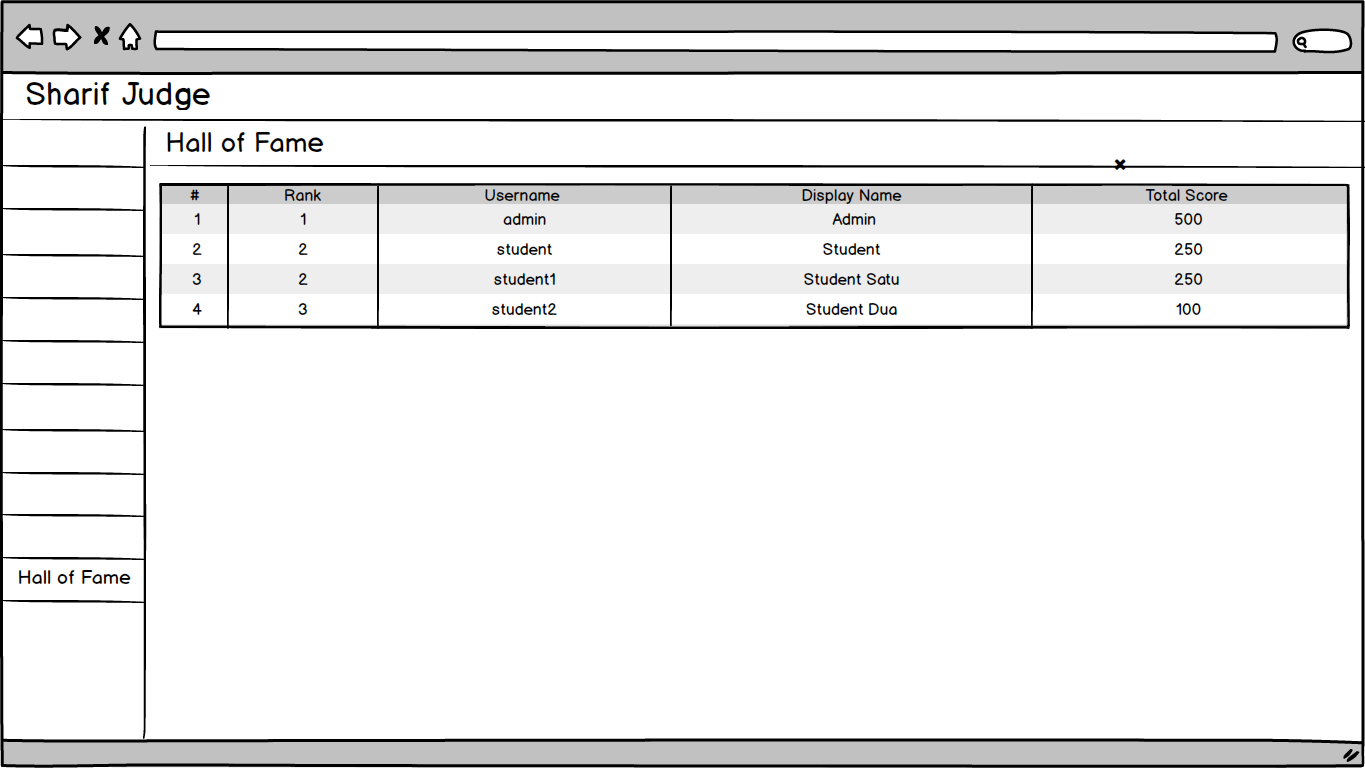
\includegraphics[width=1.0\textwidth]{mockuphof}  
		\caption[Rancangan tampilan halaman \textit{Hall of Fame}]{Rancangan tampilan halaman \textit{Hall of Fame}} 
		\label{fig:mockuphof} 
	\end{figure}

	Berikut adalah rancangan tampilan detail dari \textit{Hall of Fame} peserta tertentu
	
	\begin{figure}[H]
		\centering  
		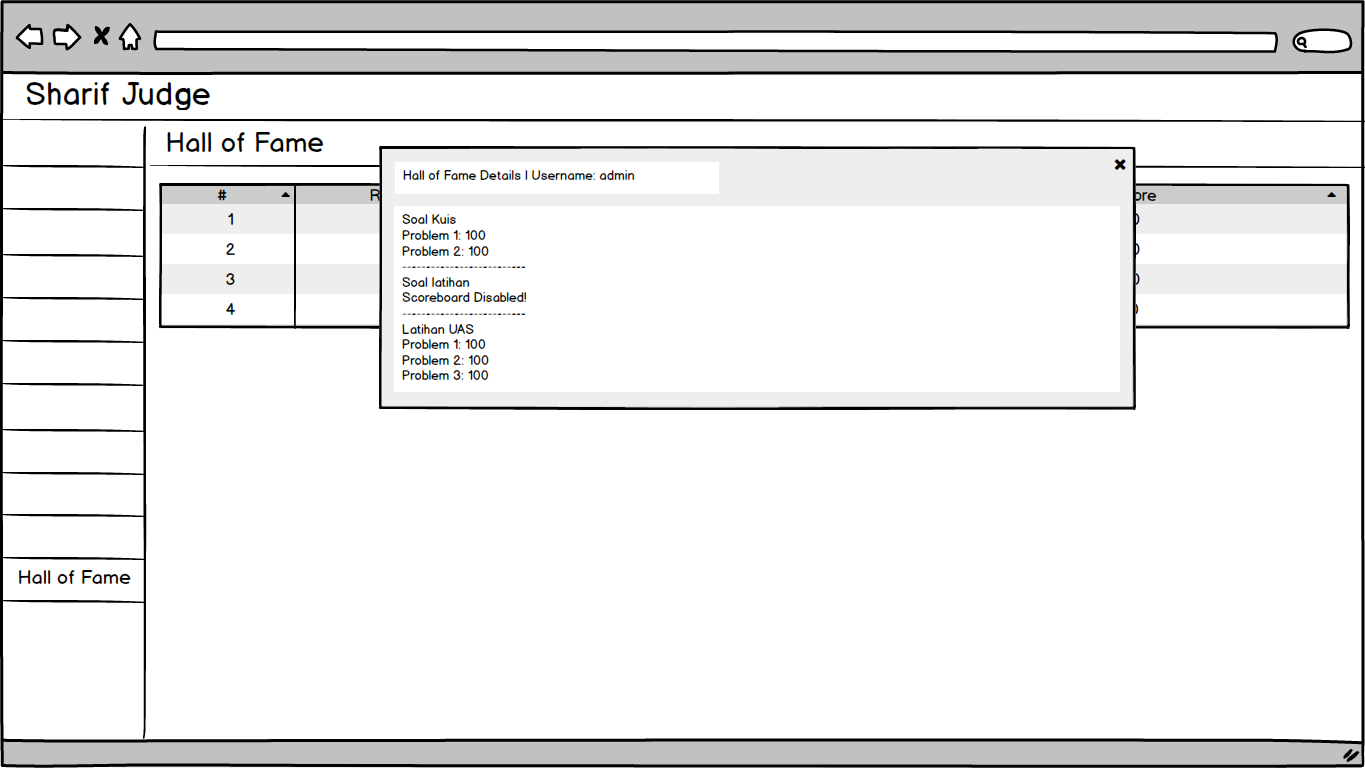
\includegraphics[width=1.0\textwidth]{mockuphofdetail}  
		\caption[Rancangan tampilan \textit{details} \textit{Hall of Fame} peserta tertentu]{Rancangan tampilan \textit{details} \textit{Hall of Fame} peserta tertentu} 
		\label{fig:mockuphofdetail} 
	\end{figure}
	
	\item \textit{Controller} \\
	\textit{Controller} untuk halaman \textit{Hall of Fame} bernama \textit{Halloffame.php}. Berikut adalah perincian fungsi yang terdapat dalam rancangan \textit{controller Logs.php}.
	\begin{table}[H]
		\caption{Perincian fungsi \textit{consturct\_\_}}
		\begin{tabular}{|c|p{11cm}|}
			\hline
			Nama \textit{Method} 	& 	\textit{consturct\_\_} 	\\
			\hline
			Parameter \textit{Input} & - \\
			\hline
			Parameter \textit{Output} &  - \\
			\hline
			Tabel yang berhubungan & - \\
			\hline
			Deskripsi	& membatasi pengguna yang dapat mengakses halaman \textit{Hall of Fame}	 \\
			\hline
			Algoritma	& \begin{itemize}
				\item mengecek \textit{session} pengguna yang akan mengakses halaman \textit{Hall of Fame}.
				\item Jika \textit{session} tidak berstatus '\textit{logged\_in}, maka pengguna akan dialihkan ke halaman \textit{login}.
				\item Memuat \textit{model Hof\_model.php}.
			\end{itemize} \\
			\hline
		\end{tabular}
	\end{table}
	
	\begin{table}[H]
		\caption{Perincian fungsi \textit{index}}
		\begin{tabular}{|c|p{11cm}|}
			\hline
			Nama \textit{Method} 	& 	\textit{index} 	\\
			\hline
			Parameter \textit{Input} & - \\
			\hline
			Parameter \textit{Output} &  - \\
			\hline
			Tabel yang berhubungan & \textit{shj\_submissions} \\
			\hline
			Deskripsi	& Proses untuk memuat seluruh entri \textit{submissions} yang telah dijumlahkan pada halaman \textit{halloffame.twig}	 \\
			\hline
			Algoritma	& \begin{itemize}
				\item Memuat data \textit{Hall of Fame} menggunakan fungsi \textit{get\_all\_final\_submission} dari \textit{model Hof\_model.php}.
				\item Memproses data untuk tampilan \textit{halloffame.twig}.
			\end{itemize} \\
			\hline
		\end{tabular}
	\end{table}
	
	\begin{table}[H]
		\caption{Perincian fungsi \textit{hof\_details}}
		\begin{tabular}{|c|p{11cm}|}
			\hline
			Nama \textit{Method} 	& 	\textit{hof\_details} 	\\
			\hline
			Parameter \textit{Input} & - \\
			\hline
			Parameter \textit{Output} &  - \\
			\hline
			Tabel yang berhubungan & \textit{shj\_submissions} \\
			\hline
			Deskripsi	& Proses untuk memuat details \textit{submissions} pada halaman \textit{halloffame.twig}	 \\
			\hline
			Algoritma	& \begin{itemize}
				\item Memuat \textit{details} \textit{Hall of Fame} peserta tertentu menggunakan fungsi \textit{get\_all\_user\_assignments} dari \textit{model Hof\_model.php}.
				\item Memproses data untuk tampilan \textit{details} \textit{Hall of Fame} dari peserta tertentu pada halaman \textit{halloffame.twig}.
			\end{itemize} \\
			\hline
		\end{tabular}
	\end{table}
\end{enumerate}

Selain menambahkan kelas \textit{model, view} dan \textit{controller}, terdapat penambahan fungsi pada \textit{file shj\_functions.js} yang terletak di \path{Sharif-Judge\assets\js}. Penambahan fungsi tersebut berguna untuk meminta \textit{details} dari Hall of Fame peserta tertentu menggunakan fungsi hof\_details pada \textit{controller Halloffame.php} lalu menampilkannya.
Berikut beberapa baris potongan kode program

\textit{shj\_functions.js}
\begin{lstlisting}[basicstyle=\ttfamily, frame=single,
columns=fullflexible, keepspaces=true, breaklines=true]
...
478	});
479
480
481
482	/**
483	* Set dir="auto" for all input elements
484	*/
485	$(document).ready(function(){
486		$('input').attr('dir', 'auto');
487	});
...
\end{lstlisting}

Fungsi tersebut ditambahkan setelah baris 479. Berikut hasil penambahan kode program yang terjadi di \textit{shj\_functions.js}
\iffalse
\textit{shj\_functions.js}
\begin{lstlisting}[basicstyle=\ttfamily, frame=single,
columns=fullflexible, keepspaces=true, breaklines=true]
...
478	});
479	
480	/**
481	* "Hall of Fame" page
482	*/
483	$(document).ready(function(){
484		$('.hof_details').click(function(){
485			var row = $(this).closest("tr");    // Find the row
486			var username = row.find(".username").text();
487			$.ajax({
488			type: 'POST',
489			url: shj.site_url+'halloffame/hof_details',
490			data: {
491				username: username,
492				shj_csrf_token: shj.csrf_token
493			},
494			beforeSend: shj.loading_start,
495			complete: shj.loading_finish,
496			error: shj.loading_error,
497	
498			success: function(response){
499				var currentAssignment = '';
500				var prevAssignment = '';
501				var temp = '';
502	
503				for (var i = 0; i < response.length; i++) {
504					if (response[i].scoreboard == 0) {
505						temp = temp + '--------------------------------------------------<br><b>' + response[i].assignment + '</b><br>Scoreboard Disabled!';
506					}
507					else{
508						if (i == 0) {
509							temp = temp + '<b>' + response[i].assignment + '</b> <br>' + response[i].problem + ' : ' + response[i].score +'<br>';
510							prevAssignment = response[i].assignment;
511						}
512						else{
513							currentAssignment = response[i].assignment;
514							var index = currentAssignment.localeCompare(prevAssignment); //comparing previous assignment's name with current assignment's name
515							if (index == 0) {
516							temp = temp + response[i].problem + ' : ' + response[i].score + '<br>';
517							prevAssignment = currentAssignment;
518							}
519							else{
520							temp = temp + '--------------------------------------------------<br><b>'+currentAssignment + '</b><br>' + response[i].problem + ' : ' + response[i].score + '<br>';
521							prevAssignment = currentAssignment;
522						}
523					}
524				}
525			}
526	
527			noty({
528				text: 'Hall of Fame for username: <b>'+username+'</b><br>============================<br>'+temp,
529				layout: 'center',
530				type: 'confirm',
531				animation: {
532					open: {height: 'toggle'},
533					close: {height: 'toggle'},
534					easing: 'swing',
535					speed: 300
536				},
537				buttons: [
538					{addClass: 'btn shj-red', text: 'Close', onClick: function($noty){$noty.close();}}
539				]
540				});
541			}
542			});
543		});
544	});
545	
546	
547	
548	/**
549	* Set dir="auto" for all input elements
550	*/
551	$(document).ready(function(){
552		$('input').attr('dir', 'auto');
553	});
...
\end{lstlisting}
\fi

\section{Integrasi \textit{Login} ke \textit{Server RADIUS}}
\textit{Sharif Judge} memerlukan \textit{library} baru agar dapat mengintegrasikan \textit{login} ke \textit{server RADIUS}. \textit{Library} yang digunakan adalah \textit{Dapphp/Radius}. \textit{Dapphp/Radius} adalah klien \textit{RADIUS PHP} untuk mengautentikasi pengguna terhadap \textit{server RADIUS} REFRENSI. Cara yang disarankan untuk menginstal \textit{Dapphp/Radius} adalah menggunakan \textit{Composer}. Jika \textit{Composer} telah terinstall, maka jalankan perintah "\textit{composer require dapphp/radius}" atau tambahkan "\textit{dapphp/radius}" pada file \textit{composer.json} bagian "\textit{section}"~\cite{drew:16:radius}.

Rancangan algoritma yang digunakan untuk menambahkan mengintegrasikan \textit{login} ke \textit{server RADIUS} yaitu
\begin{enumerate}
	\item Menginstall \textit{Composer} pada perangkat lunak \textit{Sharif Judge}.
	\item Menambahkan \textit{library Dapphp/Radius} menggunakan \textit{Composer}.
	\item Membuat \textit{file secrets.php} pada direktori \path{Sharif-Judge\application\config} untuk menyimpan configurasi alamat \textit{server RADIUS}.
	\item Mengintegrasikan \textit{login} pengguna \textit{Sharif Judge} ke \textit{server RADIUS}.
\end{enumerate}

Dari rancangan algoritma yang diterapkan, terdapat penambahan kode pada kelas \textit{model User\_model.php}. Berikut beberapa baris potongan kode program

\textit{User\_model.php}
\begin{lstlisting}[basicstyle=\ttfamily, frame=single,
columns=fullflexible, keepspaces=true, breaklines=true]
...
7	defined('BASEPATH') OR exit('No direct script access allowed');
8
9	class User_model extends CI_Model
...
323	/**
324	* Validate User
325	*
326	* Returns TRUE if given username and password is valid for login
327	*
328	* @param $username
329	* @param $password
330	* @return bool
331	*/
332	public function validate_user($username, $password)
333	{
334		$this->load->library('password_hash', array(8, FALSE));
335		$query = $this->db->get_where('users', array('username' => $username));
336		if ($query->num_rows() != 1)
337			return FALSE;
338		if ($query->row()->username !== $username) // needed (because of utf8_general_ci [ci=case insensitive])
339			return FALSE;
340		if ($this->password_hash->CheckPassword($password, $query->row()->password))
341			return TRUE;
342		return FALSE;
343	}
...
\end{lstlisting}

Penambahan kode di model \textit{User\_model} untuk memanggil \textit{library Dapphp/Radius} dan mengintegrasikan \textit{login} pengguna \textit{Sharif Judge} ke \textit{server RADIUS}. Penambahan kode tersebut terjadi setelah baris 7 dan 341. Berikut hasil penambahan kode program yang terjadi di model \textit{User\_model}

\textit{User\_model.php}
\begin{lstlisting}[basicstyle=\ttfamily, frame=single,
columns=fullflexible, keepspaces=true, breaklines=true]
...
7	defined('BASEPATH') OR exit('No direct script access allowed');
8	+use Dapphp\Radius\Radius;
9
10	class User_model extends CI_Model
...
324	/**
325	* Validate User
326	*
327	* Returns TRUE if given username and password is valid for login
328	*
329	* @param $username
330	* @param $password
331	* @return bool
332	*/
333	public function validate_user($username, $password)
334	{
335		$this->load->library('password_hash', array(8, FALSE));
336		$query = $this->db->get_where('users', array('username' => $username));
337		if ($query->num_rows() != 1)
338			return FALSE;
339		if ($query->row()->username !== $username) // needed (because of utf8_general_ci [ci=case insensitive])
340			return FALSE;
341		if ($this->password_hash->CheckPassword($password, $query->row()->password))
342			return TRUE;
343
344		$this->load->config('secrets');
345		if($this->config->item('shj_authenticate') == 'radius') {
346			$client = new Radius();
347			$client->setServer($this->config->item('shj_radius')['server']) // RADIUS server address
348				->setSecret($this->config->item('shj_radius')['secret']);
349			if($client->accessRequest($username, $password))
350				return TRUE;
351		}
352		
353		return FALSE;
354	}
...
\end{lstlisting}

\section{Branding Teknik Informatika}
Branding Teknik Informatika dilakukan dengan cara mengubah seluruh logo dan ikon \textit{Sharif Judge} menggunakan logo dan ikon Teknik Informatika. Berikut logo dan ikon Teknik Informatika yang digunakan

\begin{figure}[H]
	\centering  
	
\includegraphics[scale=1]{logosmall}  
	\caption[Logo dan Ikon]{Logo dan Ikon} 
	\label{fig:logosmall} 
\end{figure} 

\begin{figure}[H]
	\centering  
	
\includegraphics[scale=1]{banner}  
	\caption[\textit{Banner Sharif Judge}]{\textit{Banner Sharif Judge}} 
	\label{fig:banner} 
\end{figure} 

Agar dapat menggunakan logo dan ikon Teknik Informatika dibutuhkan penggantian beberapa file. Beberapa \textit{file} tersebut antara lain \textit{banner.png, favicon.ico} dan \textit{logo\_small.png} yang terdapat pada \path{Sharif-Judge\assets\images}. Penggantian beberapa \textit{file} tersebut mencakup \textit{banner} pada halaman \textit{login}, icon pada \textit{title bar} dan \textit{top bar}.

Langkah-langkah yang dilakukan untuk proses branding Teknik Informatika adalah
\begin{enumerate}
	\item Menggunakan logo dan ikon Teknik Informatika pada \textit{Sharif Judge}.
	\item Mengubah nama \textit{Sharif Judge} menjadi SharIF Judge.
	\item Mengubah link dokumentasi \textit{Github Sharif Judge} menjadi \path{https://github.com/ftisunpar/Sharif-Judge}.
\end{enumerate}

Berikut tampilan \textit{Sharif Judge} yang baru
\begin{figure}[H]
	\centering  
	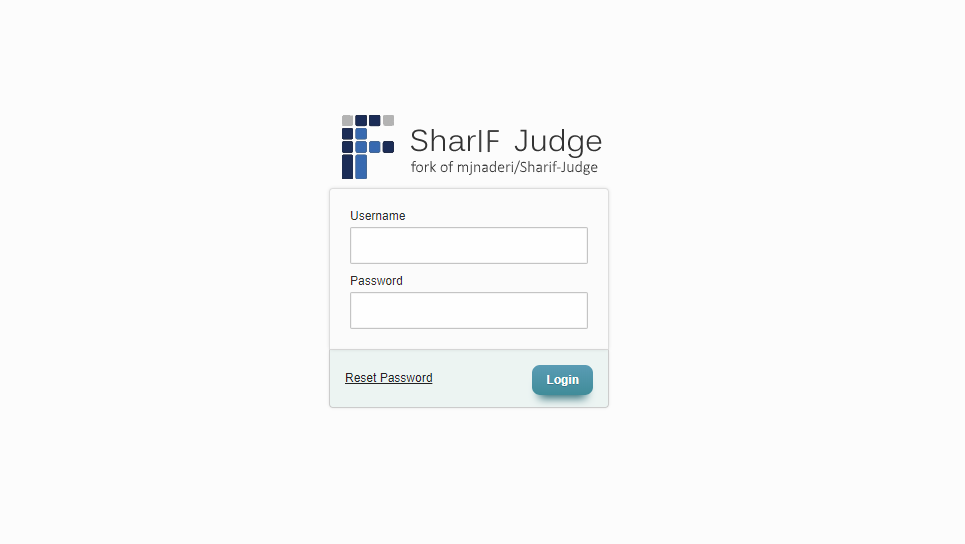
\includegraphics[scale=0.5]{login}  
	\caption[Halaman \textit{Login} \textit{Sharif Judge}]{Halaman \textit{Login} \textit{Sharif Judge}} 
	\label{fig:login} 
\end{figure}

\begin{figure}[H]
	\centering  
	
\includegraphics[scale=1]{ikon}  
	\caption[Ikon \textit{Sharif Judge} pada \textit{Title Bar}]{Ikon \textit{Sharif Judge} pada \textit{Title Bar}} 
	\label{fig:ikon} 
\end{figure} 

\begin{figure}[H]
	\centering  
	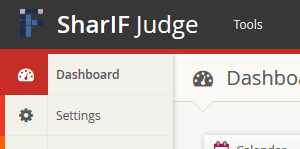
\includegraphics[scale=1]{logo}  
	\caption[Logo \textit{Sharif Judge} pada \textit{Top Bar}]{Logo \textit{Sharif Judge} pada \textit{Top Bar}} 
	\label{fig:logo} 
\end{figure} 

\section{Mengganti \textit{Library PHPExcel} Menjadi \textit{PhpSpreadsheet}}
\textit{PhpSpreadsheet} adalah \textit{library} yang ditulis dalam PHP. \textit{Library PhpSpreadsheet} menyediakan sekumpulan kelas yang memungkinkan pengguna untuk membaca dan menulis ke berbagai format \textit{file spreadsheet}, seperti \textit{Excel} dan \textit{LibreOffice Calc} ~\cite{phpoffice:10:phpspreadsheet}. Menginstall \textit{library PhpSpreadsheet} dapat dilakukan dengan menggunakan \textit{Composer} dan menjalankan perintah "\textit{composer require phpoffice/phpspreadsheet}".

Rancangan algoritma yang digunakan untuk mengganti \textit{library PHPExcel} menjadi \textit{PhpSpreadsheet} yaitu
\begin{enumerate}
	\item Menginstall \textit{Composer} pada perangkat lunak \textit{Sharif Judge}.
	\item Menambahkan \textit{library PhpSpreadsheet} menggunakan \textit{Composer}.
	\item Mengubah fungsi yang menggunakan kelas \textit{PHPExcel} menjadi menggunakan kelas \textit{PhpSpreadsheet}
\end{enumerate}

Dari rancangan algoritma yang diterapkan, terdapat perubahan kode pada kelas \textit{controller Submissions.php} dan \textit{controller Users.php}. Berikut beberapa baris potongan kode program

\textit{Submissions.php}
\begin{lstlisting}[basicstyle=\ttfamily, frame=single,
columns=fullflexible, keepspaces=true, breaklines=true]
...
7	defined('BASEPATH') OR exit('No direct script access allowed');
8
9	class Users extends CI_Controller
...
144	// Load PHPExcel library
145	$this->load->library('phpexcel');
146	
147	// Set document properties
148	$this->phpexcel->getProperties()->setCreator('Sharif Judge')
149		->setLastModifiedBy('Sharif Judge')
150		->setTitle('Sharif Judge Users')
151		->setSubject('Sharif Judge Users')
152		->setDescription('List of Sharif Judge users ('.$now.')');
153	
154	// Name of the file sent to browser
155	$output_filename = 'sharifjudge_users';
156	
157	// Set active sheet
158	$this->phpexcel->setActiveSheetIndex(0);
159	$sheet = $this->phpexcel->getActiveSheet();
...
172		'fill' => array(
173			'type' => PHPExcel_Style_Fill::FILL_SOLID,
174			'color' => array('rgb' => '173C45')
175	),
...
207		'fill' => array(
208			'type' => PHPExcel_Style_Fill::FILL_SOLID,
209			'color' => array('rgb' => (($i%2)?'F0F0F0':'FAFAFA'))
210	)
...
215	// Set text align to center
216	$sheet->getStyle( $sheet->calculateWorksheetDimension() )
217		->getAlignment()
218		->setHorizontal(PHPExcel_Style_Alignment::HORIZONTAL_CENTER);
...
228	'outline' => array(
229		'style' => PHPExcel_Style_Border::BORDER_THIN,
230		'color' => array('rgb' => '444444'),
231	),
...
249	header('Cache-Control: max-age=0');
250	$objWriter = PHPExcel_IOFactory::createWriter($this->phpexcel, ($ext==='xlsx'?'Excel2007':'Excel5'));
251	$objWriter->save('php://output');
...
\end{lstlisting}
~\\
\textit{Users.php}
\begin{lstlisting}[basicstyle=\ttfamily, frame=single,
columns=fullflexible, keepspaces=true, breaklines=true]
...
7	defined('BASEPATH') OR exit('No direct script access allowed');
8
9	class Submissions extends CI_Controller
...
58	// Load PHPExcel library
59	$this->load->library('phpexcel');
60
61	// Set document properties
62	$this->phpexcel->getProperties()->setCreator('Sharif Judge')
63		->setLastModifiedBy('Sharif Judge')
64		->setTitle('Sharif Judge Users')
65		->setSubject('Sharif Judge Users')
66		->setDescription('List of Sharif Judge users ('.$now.')');
67		
68	// Name of the file sent to browser
69	$output_filename = 'judge_'.$view.'_submissions';
70
71	// Set active sheet
72	$this->phpexcel->setActiveSheetIndex(0);
73	$sheet = $this->phpexcel->getActiveSheet();
...
99	'fill' => array(
100		'type' => PHPExcel_Style_Fill::FILL_SOLID,
101		'color' => array('rgb' => '173C45')
102	),
...
184	'fill' => array(
185		'type' => PHPExcel_Style_Fill::FILL_SOLID,
186		'color' => array('rgb' => (($i%2)?'F0F0F0':'FAFAFA'))
187	)
..
192	// Set text align to center
193	$sheet->getStyle( $sheet->calculateWorksheetDimension() )
194		->getAlignment()
195		->setHorizontal(PHPExcel_Style_Alignment::HORIZONTAL_CENTER);
...
205	'outline' => array(
206		'style' => PHPExcel_Style_Border::BORDER_THIN,
207		'color' => array('rgb' => '444444'),
208	),
...
211	header('Cache-Control: max-age=0');
212	$objWriter = PHPExcel_IOFactory::createWriter($this->phpexcel, ($ext==='xlsx'?'Excel2007':'Excel5'));
213	$objWriter->save('php://output');
...
\end{lstlisting}
~\\
Perubahan kode di controller \textit{Submissions.php} untuk mengubah fungsi yang menggunakan kelas \textit{PHPExcel} menjadi menggunakan kelas \textit{PhpSpreadsheet}. Penambahan kode tersebut terjadi setelah baris 145, 148, 158, 159, 173, 208, 218, 229 dan 250. Berikut hasil penambahan kode program yang terjadi di controller \textit{Submissions.php}

\textit{Submissions.php}
\begin{lstlisting}[basicstyle=\ttfamily, frame=single,
columns=fullflexible, keepspaces=true, breaklines=true]
...
7	defined('BASEPATH') OR exit('No direct script access allowed');
8
9	use PhpOffice\PhpSpreadsheet\Spreadsheet;
10	use PhpOffice\PhpSpreadsheet\IOFactory;
11	use PhpOffice\PhpSpreadsheet\Writer\Xlsx;
12	use PhpOffice\PhpSpreadsheet\Style\Fill;
13	use PhpOffice\PhpSpreadsheet\Style\Border;
14	use PhpOffice\PhpSpreadsheet\Style\Alignment;
15
16	class Users extends CI_Controller
...
151	// Load PHPExcel library
152	$phpspreedsheet = new Spreadsheet();
153	
154	// Set document properties
155	$phpspreedsheet->getProperties()->setCreator('SharIF Judge')
156		->setLastModifiedBy('Sharif Judge')
157		->setTitle('Sharif Judge Users')
158		->setSubject('Sharif Judge Users')
159		->setDescription('List of Sharif Judge users ('.$now.')');
160	
161	// Name of the file sent to browser
162	$output_filename = 'sharifjudge_users';
163	
164	// Set active sheet
165	$phpspreedsheet->setActiveSheetIndex(0);
166	$sheet = $phpspreedsheet->getActiveSheet();
...
179		'fill' => array(
180			'fillType' => Fill::FILL_SOLID,
181			'color' => array('rgb' => '173C45')
182	),
...
214		'fill' => array(
215			'fillType' => Fill::FILL_SOLID,
216			'color' => array('rgb' => (($i%2)?'F0F0F0':'FAFAFA'))
217	)
...
222	// Set text align to center
223	$sheet->getStyle( $sheet->calculateWorksheetDimension() )
224		->getAlignment()
225		->setHorizontal(Alignment::HORIZONTAL_CENTER);
...
235	'outline' => array(
236		'borderStyle' => Border::BORDER_THIN,
237		'color' => array('rgb' => '444444'),
238	),
...
256	header('Cache-Control: max-age=0');
257	$objWriter = IOFactory::createWriter($phpspreedsheet, ucfirst($ext));
258	$objWriter->save('php://output');
...
\end{lstlisting}
~\\
Perubahan kode di \textit{controller Users.php} untuk mengubah fungsi yang menggunakan kelas \textit{PHPExcel} menjadi menggunakan kelas \textit{PhpSpreadsheet}. Penambahan kode tersebut terjadi setelah baris 59, 72, 73, 100, 185, 195, 206 dan. Berikut hasil penambahan kode program yang terjadi di \textit{controller Users.php}

\textit{Users.php}
\begin{lstlisting}[basicstyle=\ttfamily, frame=single,
columns=fullflexible, keepspaces=true, breaklines=true]
...
7	defined('BASEPATH') OR exit('No direct script access allowed');
8
9	use PhpOffice\PhpSpreadsheet\Spreadsheet;
10	use PhpOffice\PhpSpreadsheet\IOFactory;
11	use PhpOffice\PhpSpreadsheet\Writer\Xlsx;
12	use PhpOffice\PhpSpreadsheet\Style\Fill;
13	use PhpOffice\PhpSpreadsheet\Style\Border;
14	use PhpOffice\PhpSpreadsheet\Style\Alignment;
15	class Submissions extends CI_Controller
...
65	// Load PHPExcel library
66	$phpspreedsheet = new Spreadsheet();
67	
68	// Set document properties
69	$phpspreedsheet->getProperties()->setCreator('SharIF Judge')
70		->setLastModifiedBy('Sharif Judge')
71		->setTitle('Sharif Judge Users')
72		->setSubject('Sharif Judge Users')
73		->setDescription('List of Sharif Judge users ('.$now.')');
74	
75	// Name of the file sent to browser
76	$output_filename = 'sharifjudge_users';
77	
78	// Set active sheet
79	$phpspreedsheet->setActiveSheetIndex(0);
80	$sheet = $phpspreedsheet->getActiveSheet();
...
106	'fill' => array(
107		'fillType' => Fill::FILL_SOLID,
108		'color' => array('rgb' => '173C45')
109	),
...
191	'fill' => array(
192		'fillType' => Fill::FILL_SOLID,
193		'color' => array('rgb' => (($i%2)?'F0F0F0':'FAFAFA'))
194	)
..
199	// Set text align to center
200	$sheet->getStyle( $sheet->calculateWorksheetDimension() )
201		->getAlignment()
202		->setHorizontal(Alignment::HORIZONTAL_CENTER);
...
212	'outline' => array(
213		'borderStyle' => Border::BORDER_THIN,
214		'color' => array('rgb' => '444444'),
215	),
...
218	header('Cache-Control: max-age=0');
219	$objWriter = IOFactory::createWriter($phpspreedsheet, ucfirst($ext));
220	$objWriter->save('php://output');
...
\end{lstlisting}